\documentclass{beamer}
\usetheme{metropolis}           % Use metropolis theme
%\usepackage[german]{babel}  
\usepackage[utf8]{inputenc}	%dt Sonderzeichen wie ß
\usepackage{tikz}
\usepackage{amssymb}
\usepackage{multirow}
\usepackage{pgfpages}
\usepackage{cite}
\usepackage{graphicx}
\usepackage{animate}


\usepackage{multimedia}
\usepackage{float}
\usepackage{subfig}
\usepackage{svg}
\usepackage{enumitem}


%\setbeameroption{show notes on second screen=right}  %% Uncomment this to get Notes


%\renewcommand*{\figurename}{Abb.}




\title{A configurable speech recognition pipeline for social robots}
\subtitle{Creating a fusion framework for analyzing speech data}
\date{11.7.2019}
\institute{
	Master Thesis\\
	\begin{tabular}[t]{@{}l@{\hspace{3pt}}p{.32\textwidth}@{}}
		Supervisiors: & Sven Wachsmuth \\
		& Florian Lier \\
		& Birte Carlmeyer
	\end{tabular}%
	\begin{tabular}[t]{@{}l@{\hspace{3pt}}p{.3\textwidth}@{}}
		Reviewers: & Sven Wachsmuth \\
		& Florian Lier
	\end{tabular}%
	}
\author{Robert Feldhans}



%TODO:
% add metadata to title

\begin{document}
	\maketitle
	
	\begin{frame}{Content}
		\setbeamertemplate{section in toc}[sections numbered]
		\tableofcontents[hideallsubsections]
	\end{frame}
	
	
	
	
	
	
	
	\section{Motivation}
	
	\begin{frame}{Foray Robocup Speechrec Task}
		\centering
		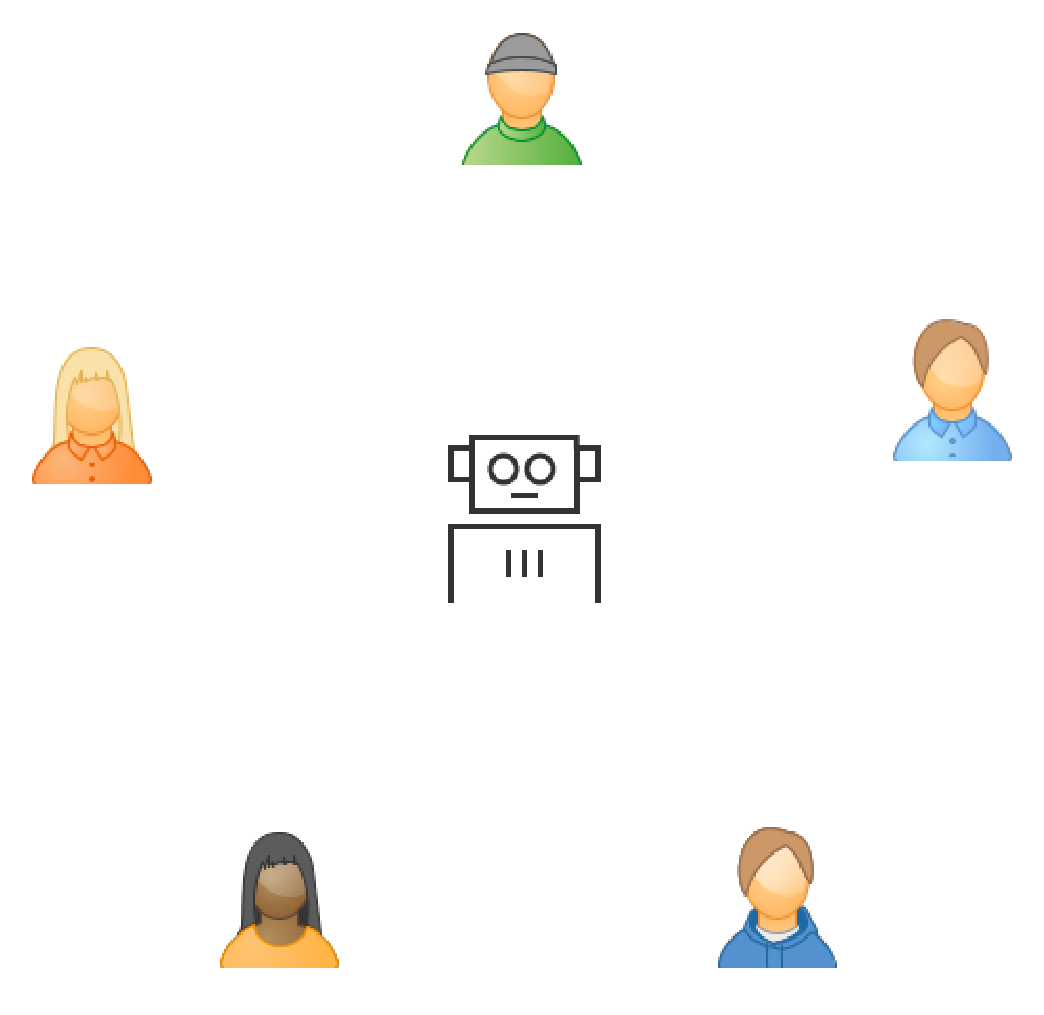
\includegraphics[width=.75\textwidth]{Bilder/robocup_task}
	\end{frame}
	
	\begin{frame}{Foray Robocup Speechrec Task}
		\centering
		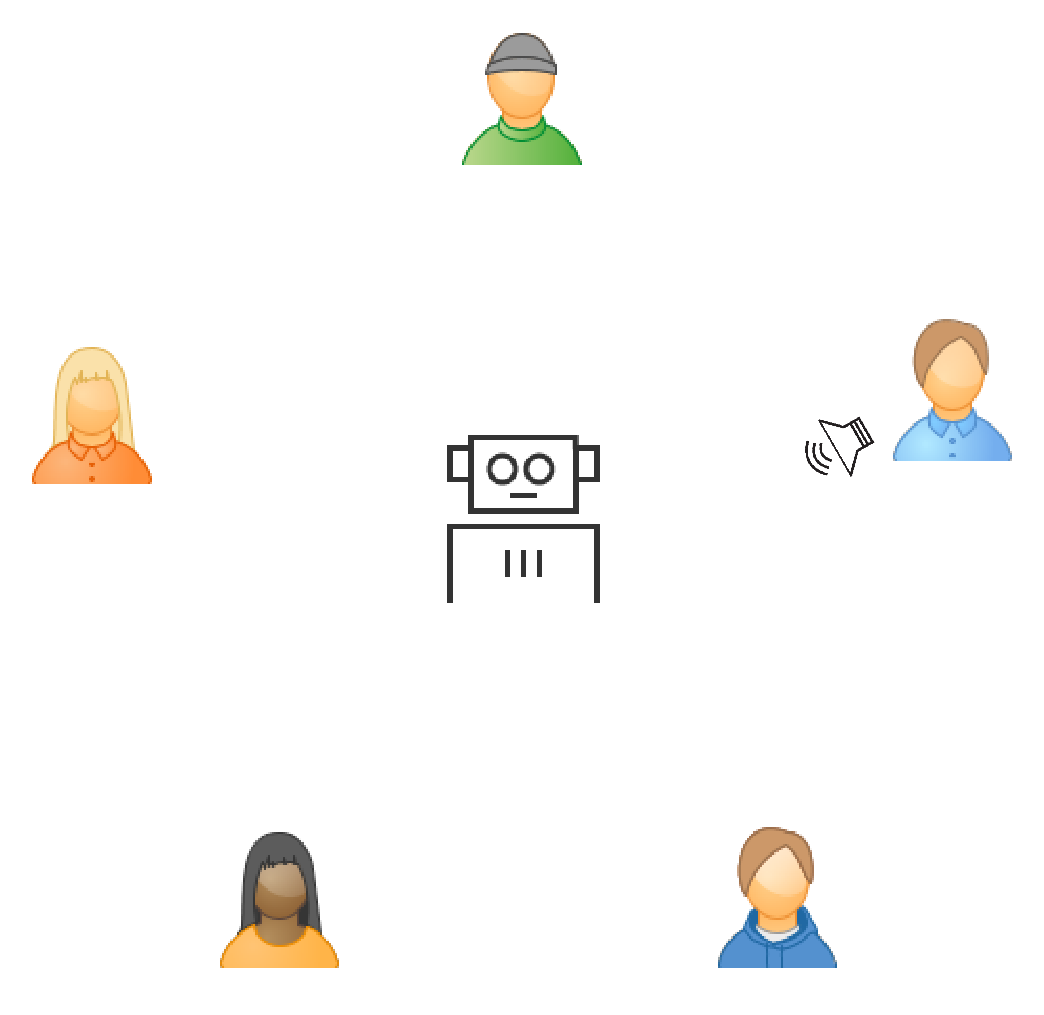
\includegraphics[width=.75\textwidth]{Bilder/robocup_task_1}
	\end{frame}
	
	\begin{frame}{Foray Robocup Speechrec Task}
		\centering
		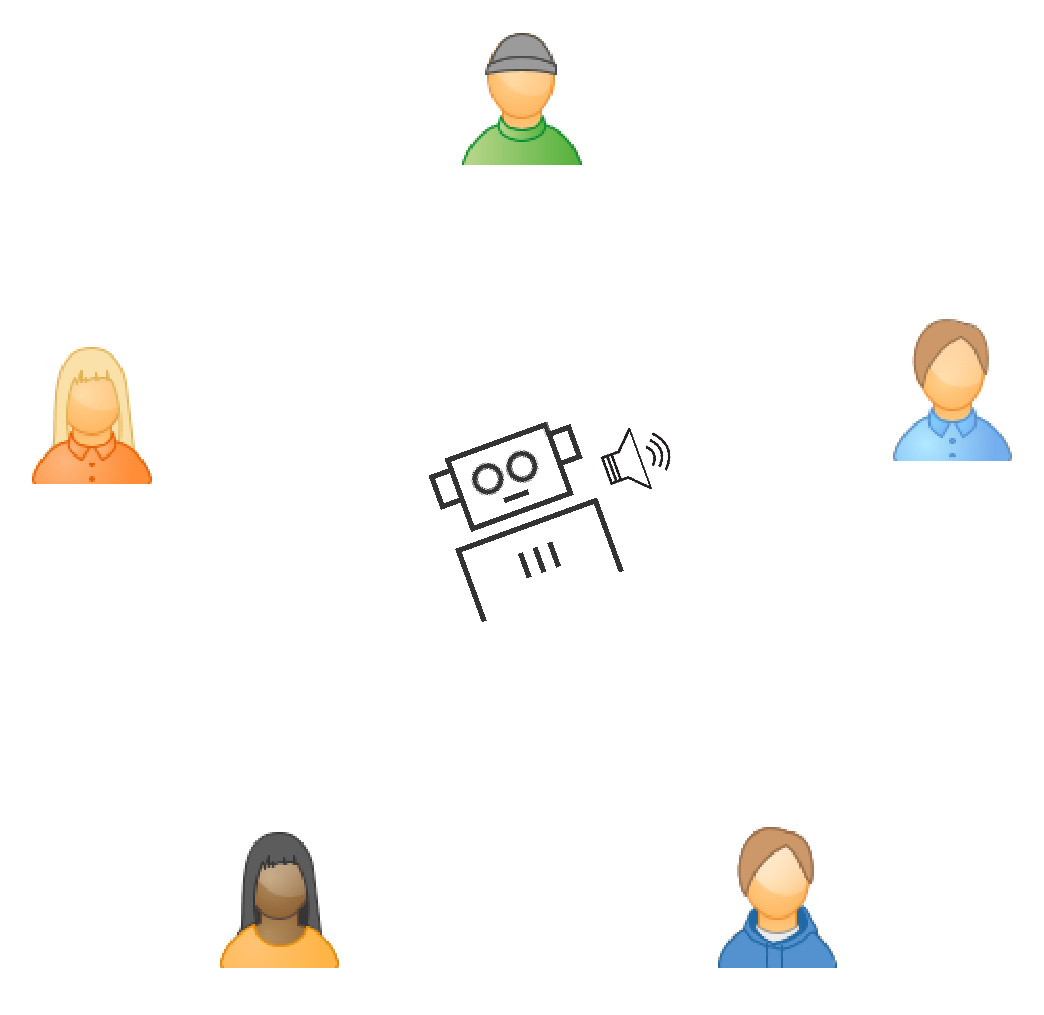
\includegraphics[width=.75\textwidth]{Bilder/robocup_task_2}
	\end{frame}
	
	\begin{frame}{Foray Robocup II}
		\centering
		\movie[width=\textwidth,poster,autostart,showcontrols,loop]{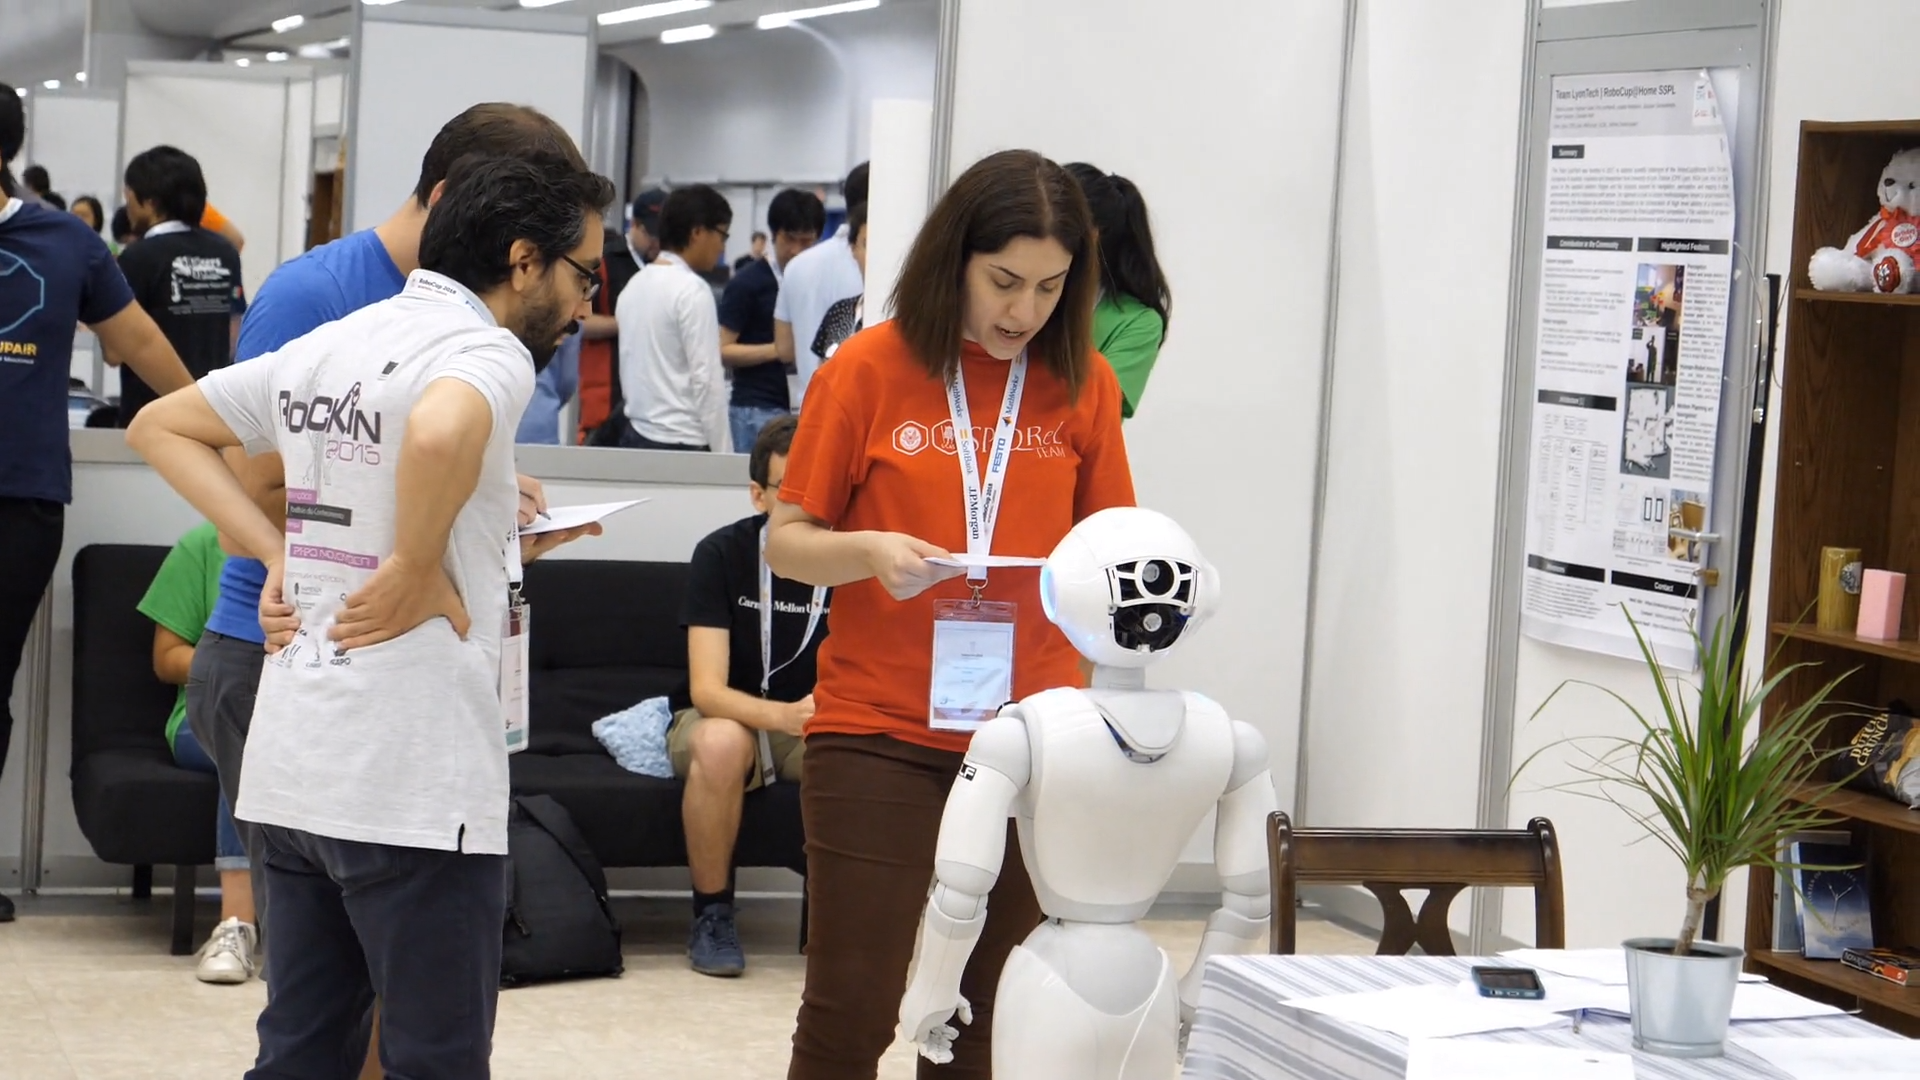
\includegraphics[width=\textwidth]{Bilder/robocup.png}}{Bilder/robocup.mp4}
	\end{frame}
	
	\begin{frame}{Robocup}
		
		\begin{alertblock}{What are requirements for a robot regarding speech recognition? What is nice to have? What would be the optimum?}
			\pause
			\begin{itemize}
				\item[-] Robustness (especially regarding noise)
				\item[-] Beamforming / Signal enhancing
				\item[-] Modularity
				\item[-] Synchronization
			\end{itemize}
		\end{alertblock}
		
	\end{frame}
	
	
	\begin{frame}{Additional Thoughts}
		\begin{alertblock}{With these requirements set, what can we get for free?}
			\pause
			\begin{itemize}
				\item[-] Gender Recognition
				\item[-] Emotion Recognition
				\item[-] Voice Recognition
				\item[-] Signal Enhancing
			\end{itemize}
			\pause
			Synchronization can be used to fuse all this information!
		\end{alertblock}
	\end{frame}
	
	\begin{frame}{Foray: Latency vs Signal Integrity}
		\begin{alertblock}{Latency}
			\begin{itemize}
				\item[-] Important for humans, stuttering makes recognition hard!
				\item[-] Not that important for machines, as they can wait till they get the full signal
			\end{itemize}
		\end{alertblock}
		\pause
		\begin{alertblock}{Signal Integrity}
			\begin{itemize}
				\item[-] Definitely recognizable by humans, but we can deal with it
				\item[-] Important for machines, otherwise artifacts may occur!
			\end{itemize}
		\end{alertblock}
	\end{frame}
	
	\begin{frame}{Artifacts}
		content...
		%todo: diagram
	\end{frame}
	
	\begin{frame}{Artifacts II}
		content...
		%todo: audio files
	\end{frame}
	
	
	\begin{frame}{Evaluation of existing solutions}
		\begin{alertblock}{ALSA/ Pulseaudio}
			\begin{itemize}
				\item[-] Available everywhere
				\item[-] Lack options for easy audio in- \& output
				\item[-] Timestamping/ adding custom meta information is basically impossible
			\end{itemize}
		\end{alertblock}
		\pause
		\begin{alertblock}{Jack Audio/ Gstreamer}
			\begin{itemize}
				\item[-] strong focus on real time audio
				\item[-] Timestamping/ adding custom meta information is basically impossible
			\end{itemize}
		\end{alertblock}
	\end{frame}
	
	
	
	
	
	

	\section{Pipeline}
	
	\begin{frame}{Idea}
		
	\end{frame}
	
	\begin{frame}{Augmented audio}
		\centering
		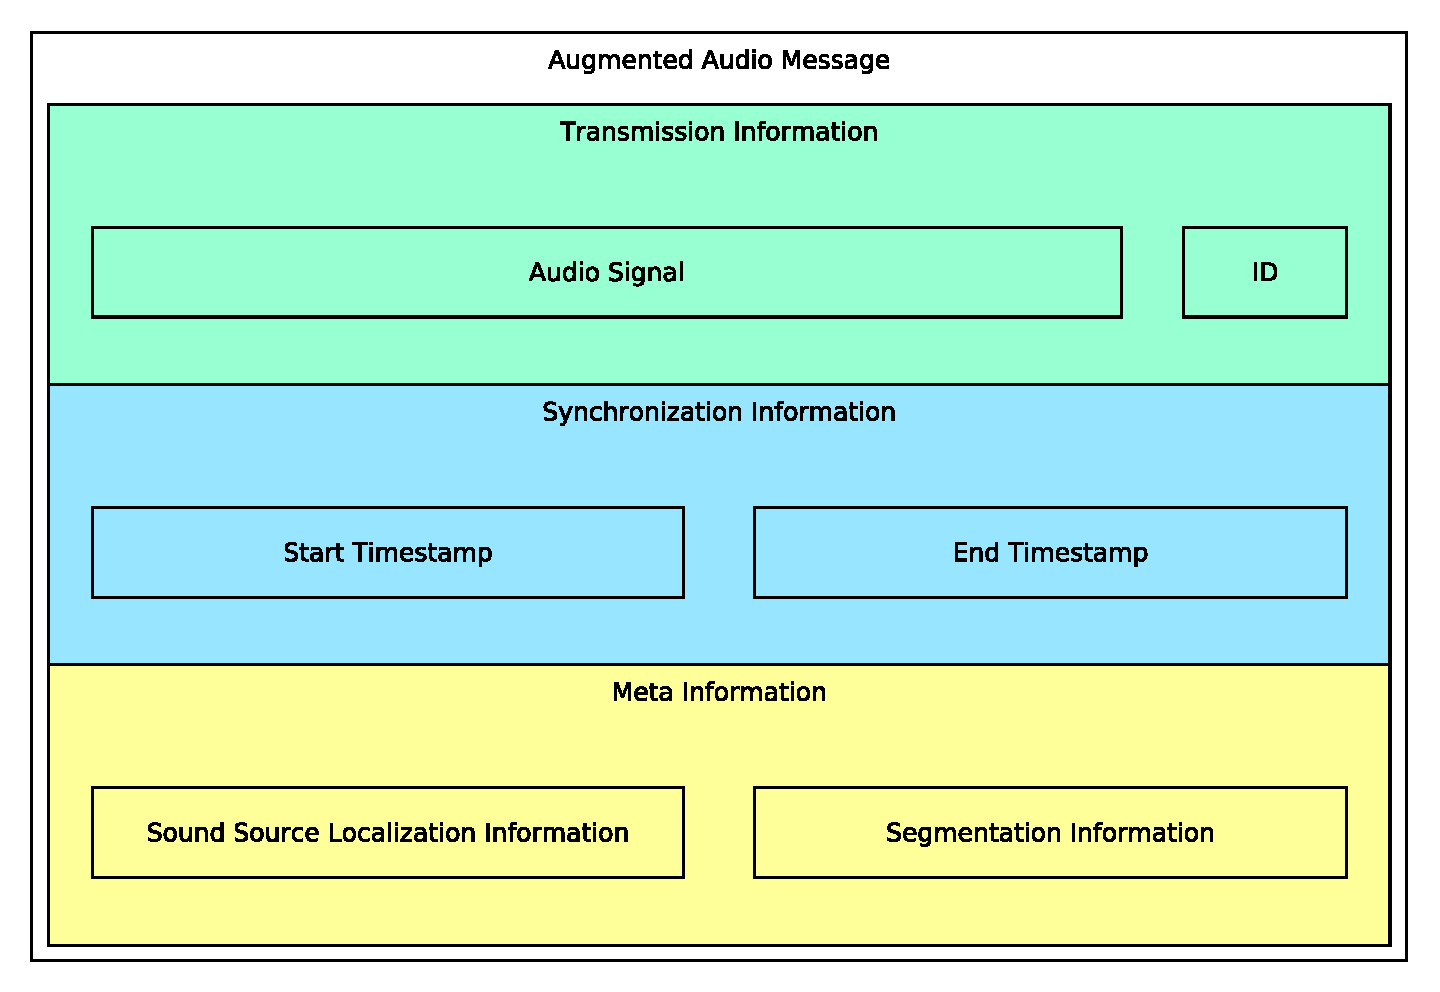
\includegraphics[width=\textwidth]{Bilder/augmented_audio}
	\end{frame}
	
	\begin{frame}{Architecture (Sound)}
		\centering
		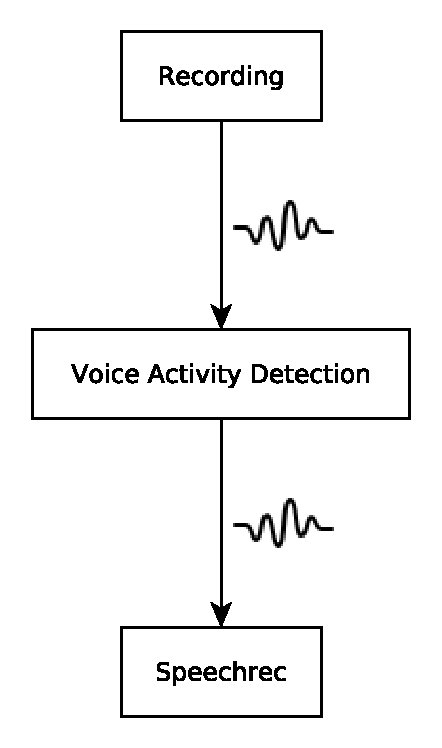
\includegraphics[width=.40\textwidth]{Bilder/audio_flow}
	\end{frame}
	
	\begin{frame}{Architecture (Sound)}
		\centering
		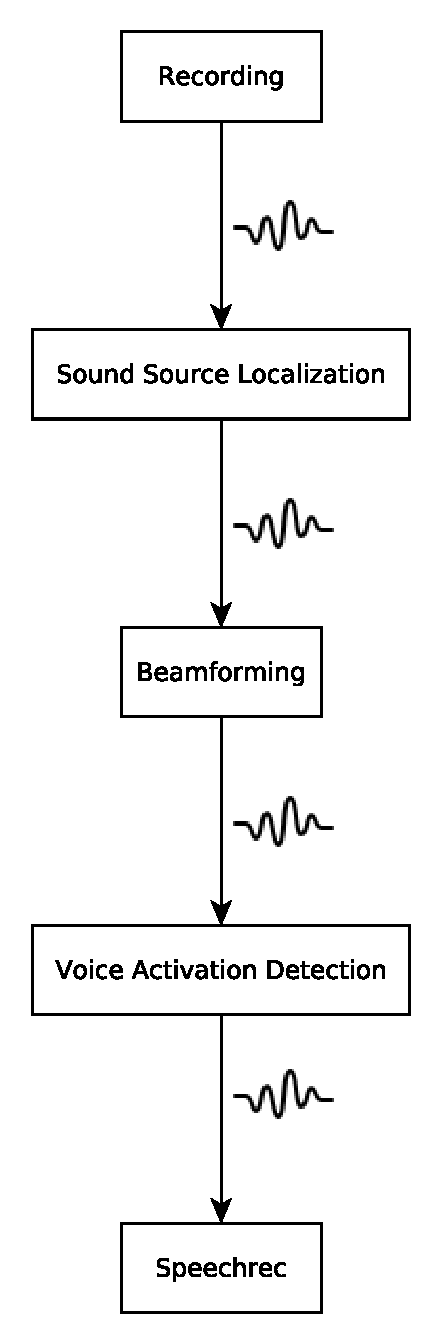
\includegraphics[height=8cm]{Bilder/audio_flow_1}
	\end{frame}
	
	\begin{frame}{Architecture (Sound)}
		\centering
		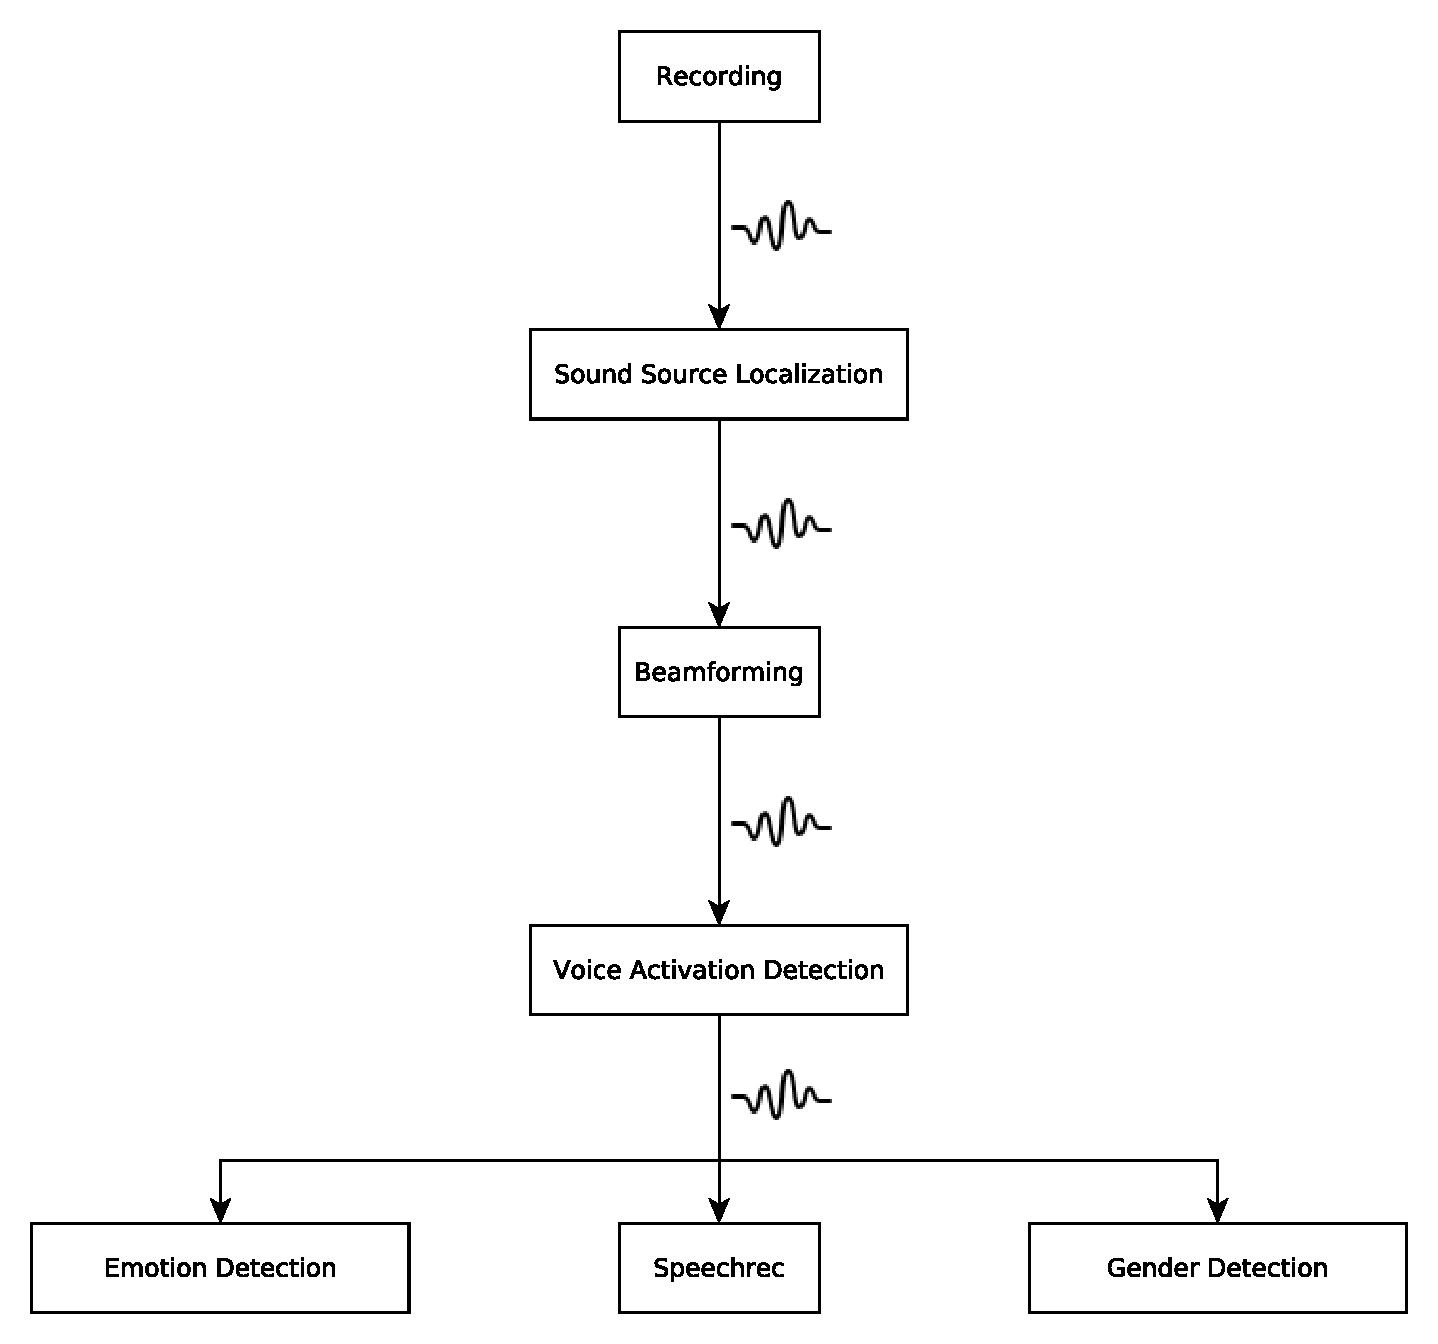
\includegraphics[height=8cm]{Bilder/audio_flow_2}
	\end{frame}
	
	\begin{frame}{Architecture (Information)}
		\centering
		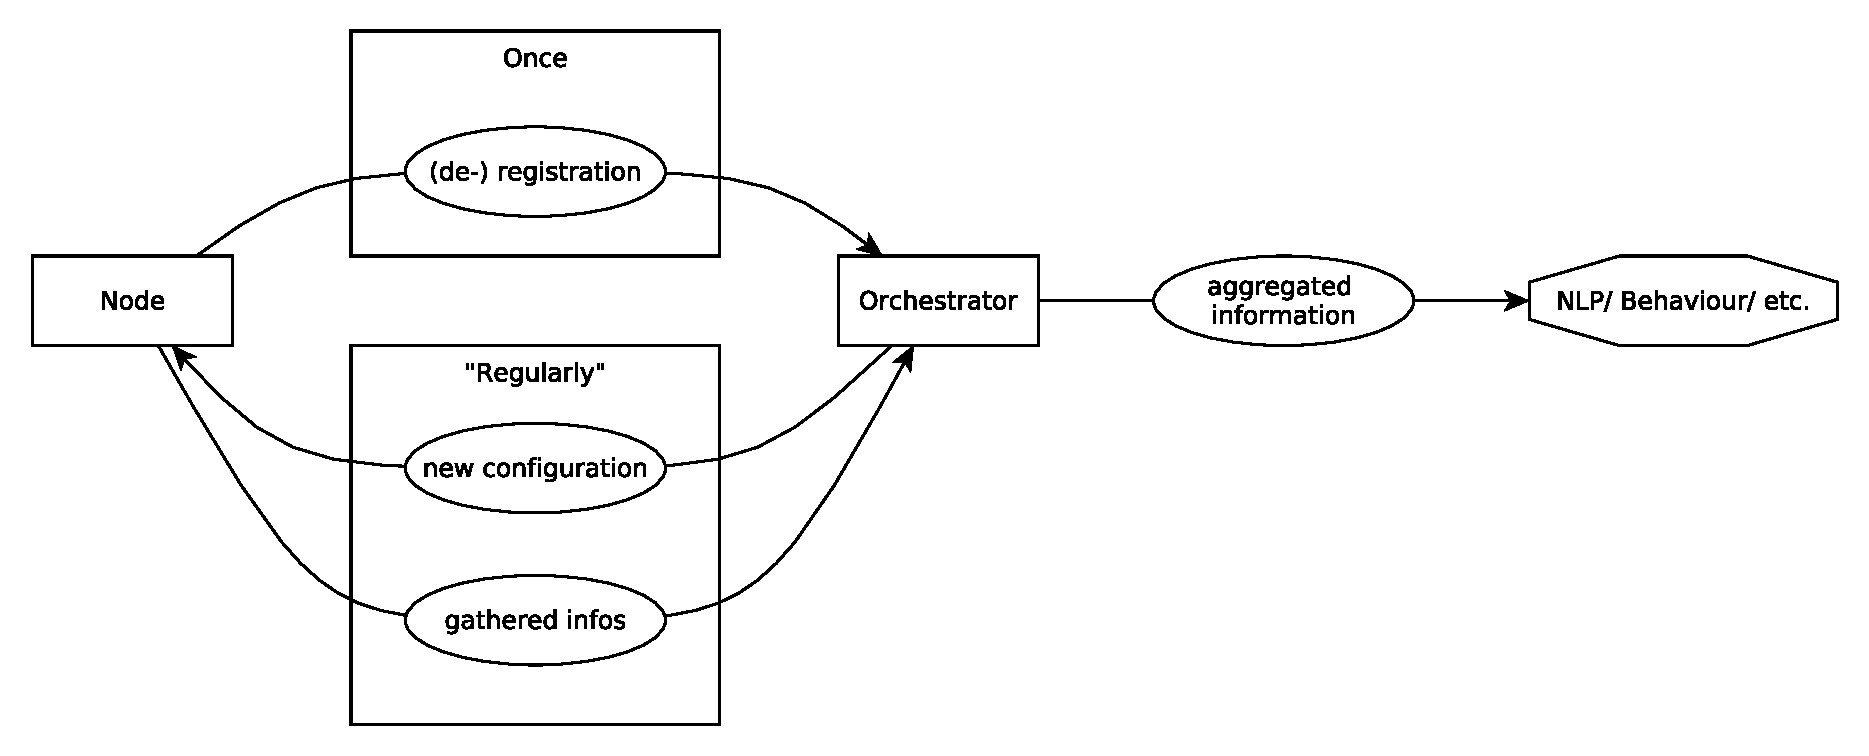
\includegraphics[width=\textwidth]{Bilder/orchestrator}
	\end{frame}
	
	
	
	
	
	
	
	
	\section{Current State}
	\begin{frame}{Progress}
		\centering
		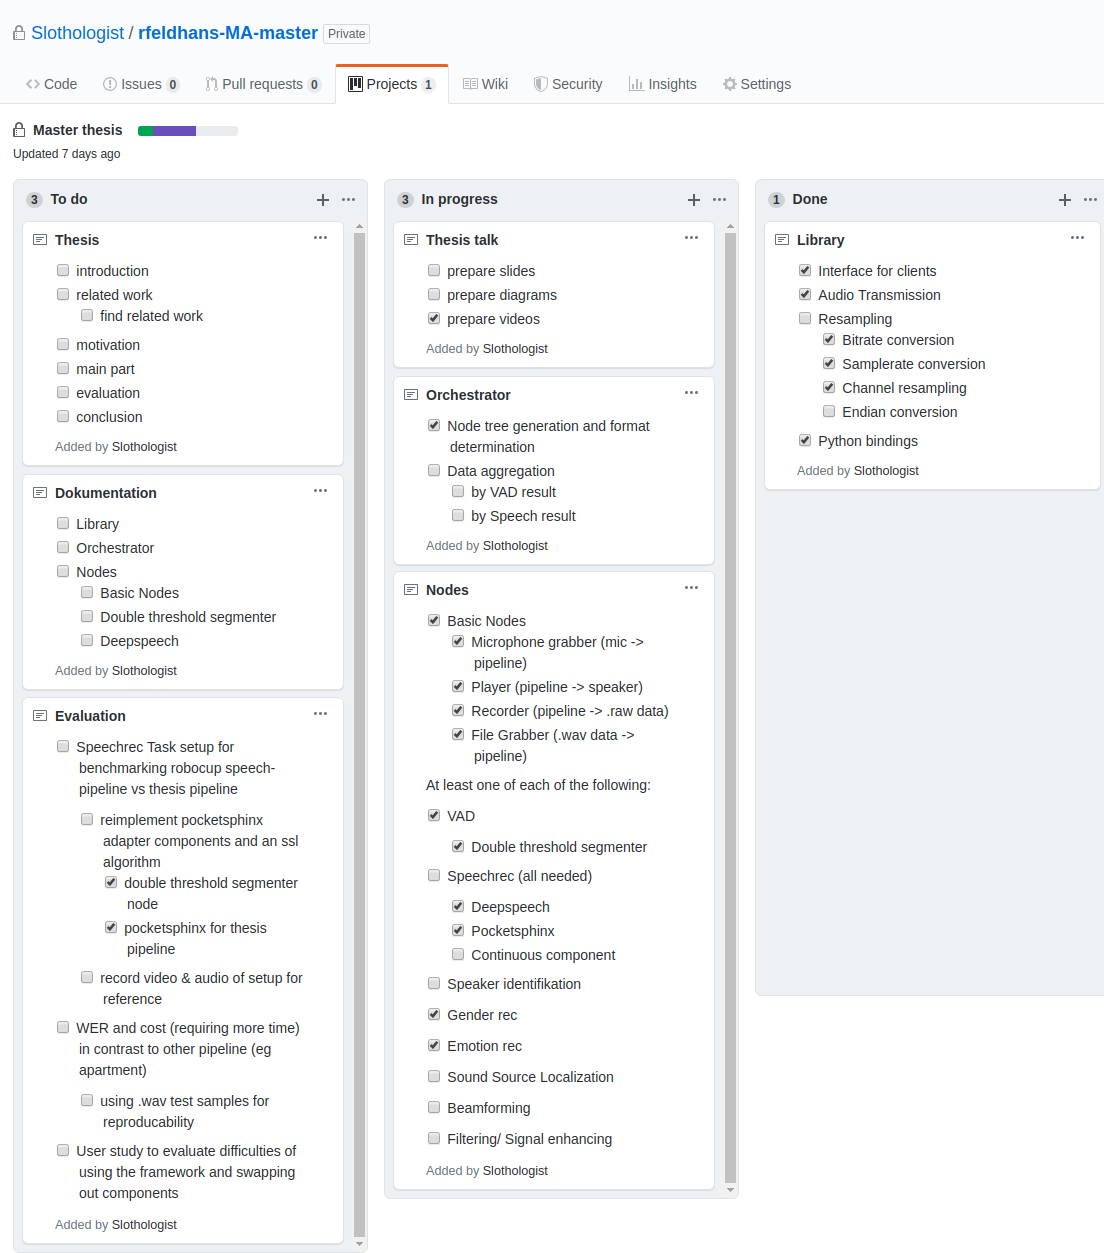
\includegraphics[height=8cm]{Bilder/progress}
	\end{frame}
	
	
	
	
	
	
	
	
	
	\section{Evaluation}
	
	\begin{frame}{Robocup Speechrec Task}
		\pause
		Pros:
		\begin{itemize}
			\item[-] is widely used to test robots speech recognition capabilities
			\item[-] score can be used to compare against dozens of other robots
		\end{itemize}
		\pause
		Cons:
		\begin{itemize}
			\item[-] setup (noise) is a bit tricky, but can be adequately simulated using several speakers in a big echoing hall
			\item[-] is somewhat random, because some questions may be more difficult than others (however, difficulty may depend on components)
			\item[-] encompasses a bit of visual person recognition as well as ''NLP'', but both are irrelevant for us
		\end{itemize}
	\end{frame}
	
	\begin{frame}{Dataset Evaluation}
		Everything is modular, so even the input can be switched out, so just read wav files instead of microphone input.\\

		Compare WER and CPU/ overall time between...
		\begin{itemize}
			\item[-] bare minimum pipeline
			\item[-] ''longer'' pipeline (more preprocessing)
			\item[-] ''wider'' pipeline (more parallel components)
			\item[-] all encompassing pipeline
			\item[-] other pipelines (e.g. apartment)
		\end{itemize}
	\end{frame}
	
	\begin{frame}{Fusion Test}
		\centering
		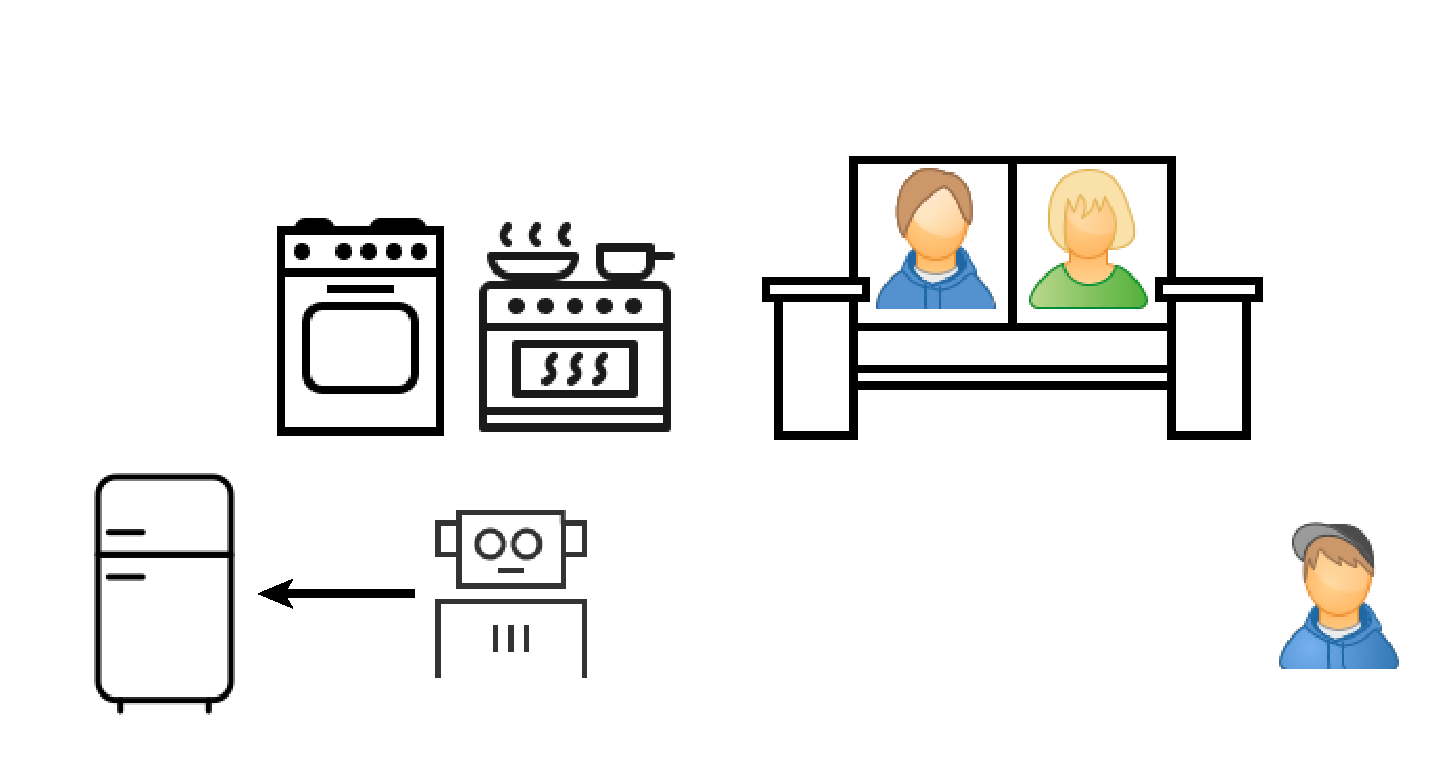
\includegraphics[width=.75\textwidth]{Bilder/fusion_test_0}
	\end{frame}
	
	\begin{frame}{Fusion Test}
		\centering
		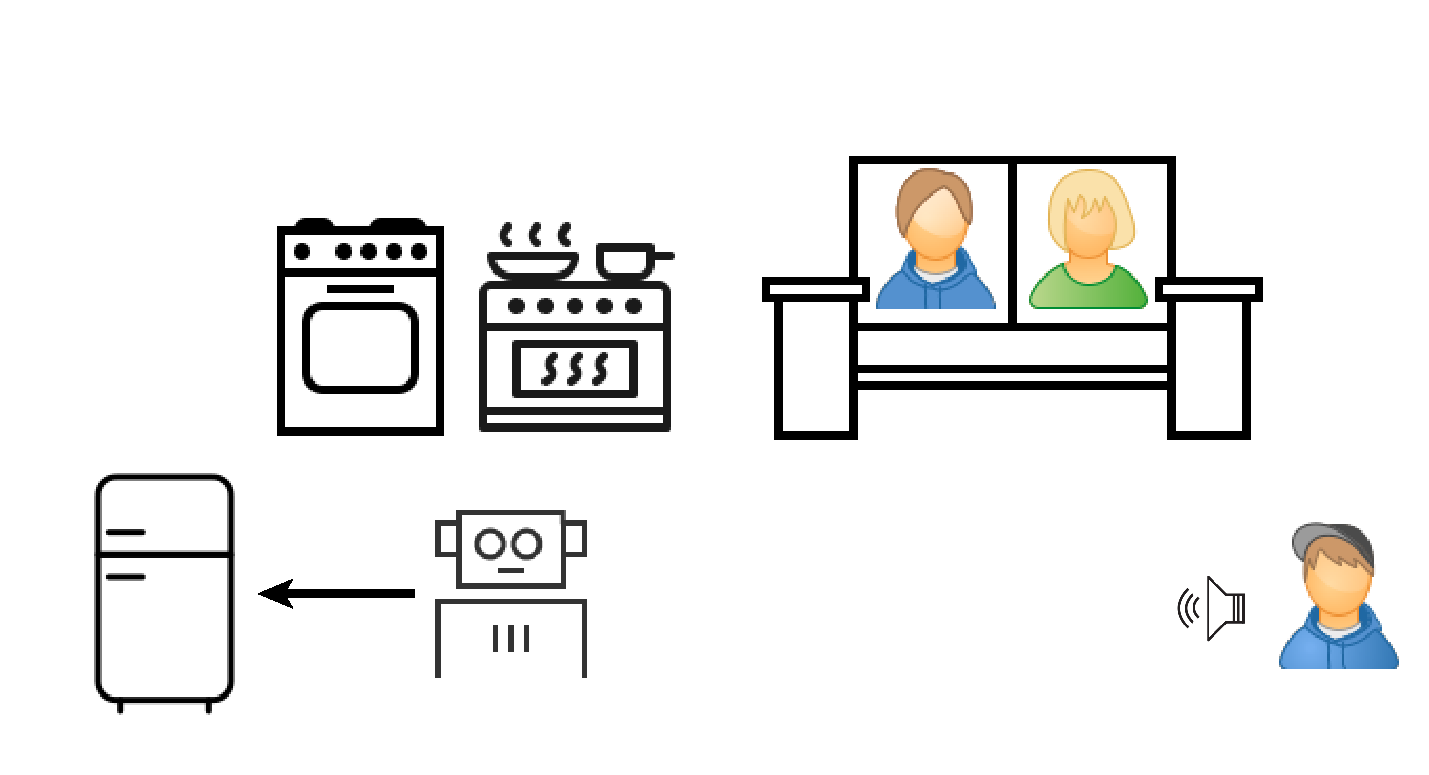
\includegraphics[width=.75\textwidth]{Bilder/fusion_test_1}
	\end{frame}
	
	\begin{frame}{Fusion Test}
		\centering
		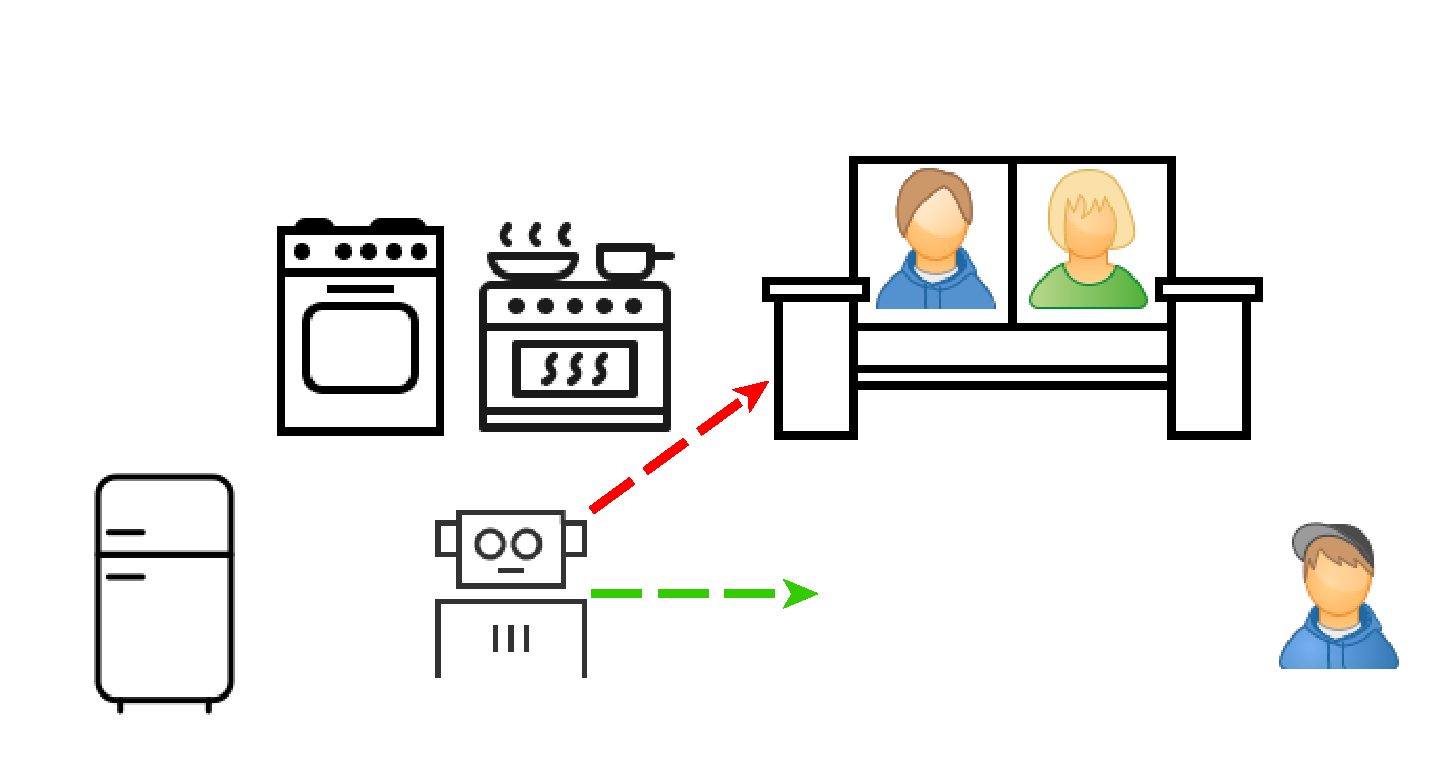
\includegraphics[width=.75\textwidth]{Bilder/fusion_test_2}
	\end{frame}
	
	\begin{frame}{Fusion Test}
		\begin{alertblock}{What to evaluate with this test?}
			\pause
			\begin{itemize}
				\item[-] qualitative analysis
				\item[-] TODO
			\end{itemize}
		\end{alertblock}
	\end{frame}
	
	
	
	
	
	\section{Demo}
	
	\begin{frame}{Demo Backup: Video}
		%\centering
		%\movie[width=\textwidth,poster,autostart,showcontrols,loop]{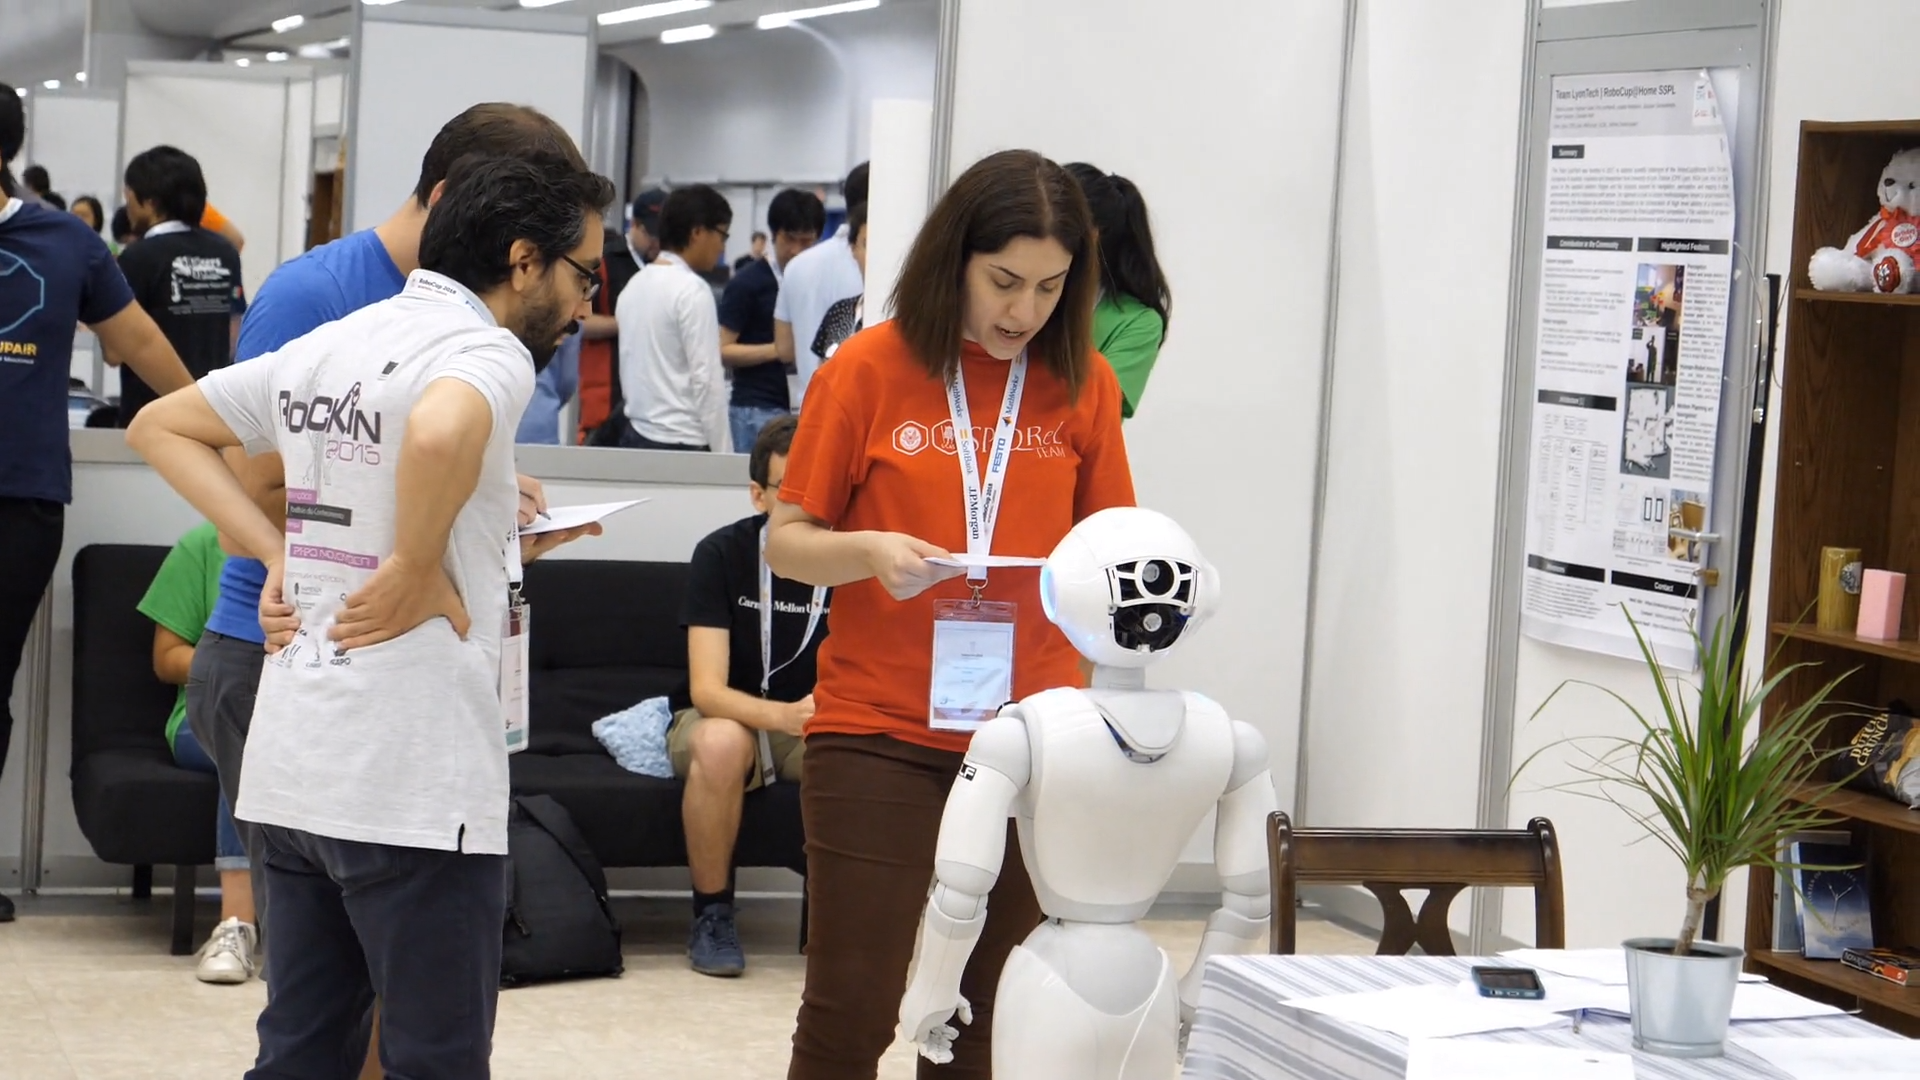
\includegraphics[width=\textwidth]{Bilder/robocup.png}}{Bilder/robocup.mp4}
	\end{frame}
	
	
	
	\begin{frame}{}
		\begin{alertblock}{Thanks for your Attention!}
		\end{alertblock}
	\end{frame}
	
	\begin{frame}{}
		\begin{alertblock}{Discussion}
		\end{alertblock}
	\end{frame}
	
\end{document}
	
	
	